\everymath{\displaystyle}
\documentclass{beamer}
% \documentclass[handout]{beamer}

%\usepackage[pdftex]{color,graphicx}
\usepackage{amsmath,amssymb,amsfonts}

\mode<presentation>
{
  % \usetheme{Darmstadt}
  % \usetheme[hideothersubsections]{Hannover}
  % \usetheme[hideothersubsections]{Goettingen}
  \usetheme[hideothersubsections, right]{Berkeley}

  \usecolortheme{seahorse}
  % \usecolortheme{dolphin}
  \usecolortheme{rose}
  % \usecolortheme{orchid}

  \useinnertheme[shadow]{rounded}

  \setbeamercovered{transparent}
  % or whatever (possibly just delete it)
}

\mode<handout>{
  \setbeamercolor{background canvas}{bg=black!5}
  \usepackage{pgfpages}
  \pgfpagesuselayout{4 on 1}[a4paper,border shrink=5mm, landscape]
}

\usepackage[brazilian]{babel}
% or whatever

% \usepackage[latin1]{inputenc}
\usepackage[utf8]{inputenc}
% or whatever

\usepackage{times}
%\usepackage[T1]{fontenc}
% Or whatever. Note that the encoding and the font should match. If T1
% does not look nice, try deleting the line with the fontenc.


\title%[] % (optional, use only with long paper titles)
{Inferência I}

\subtitle
{Inferências com amostras grandes} % (optional)

\author%[] % (optional, use only with lots of authors)
{Felipe Figueiredo}% \and S.~Another\inst{2}}
% - Use the \inst{?} command only if the authors have different
%   affiliation.

\institute[INTO] % (optional, but mostly needed)
{Instituto Nacional de Traumatologia e Ortopedia
}
  % \inst{1}%
  % Department of Computer Science\\
  % University of Somewhere
  % \and
  % \inst{2}%
  % Department of Theoretical Philosophy\\
  % University of Elsewhere}
% - Use the \inst command only if there are several affiliations.
% - Keep it simple, no one is interested in your street address.

\date%[] % (optional)
{}

% \subject{Talks}
% This is only inserted into the PDF information catalog. Can be left
% out. 



% If you have a file called "university-logo-filename.xxx", where xxx
% is a graphic format that can be processed by latex or pdflatex,
% resp., then you can add a logo as follows:

\pgfdeclareimage[height=1.6cm]{university-logo}{../logo}
\logo{\pgfuseimage{university-logo}}



% Delete this, if you do not want the table of contents to pop up at
% the beginning of each subsection:
\AtBeginSubsection[]
%\AtBeginSection[]
{
  \begin{frame}<beamer>{Sumário}
    \tableofcontents[currentsection,currentsubsection]
  \end{frame}
}


% If you wish to uncover everything in a step-wise fashion, uncomment
% the following command: 

\beamerdefaultoverlayspecification{<+->}


\begin{document}

\begin{frame}
  \titlepage
\end{frame}

\begin{frame}{Sumário}
  \tableofcontents
  % You might wish to add the option [pausesections]
\end{frame}

%% Template
% \section{}

% \subsection{}

% \begin{frame}{}
%   \begin{itemize}
%   \item 
%   \end{itemize}
% \end{frame}

% \begin{frame}
%   \begin{columns}
%     \begin{column}{5cm}
%     \end{column}
%     \begin{column}{5cm}
%     \end{column}
%   \end{columns}
% \end{frame}

% \begin{frame}{}
%   \includegraphics[height=0.4\textheight]{file1}
%   \includegraphics[height=0.4\textheight]{file2}
%   \includegraphics[height=0.4\textheight]{file3}
%   \begin{figure}
%     \caption{}
%   \end{figure}
% \end{frame}

% \begin{frame}{}
%   \begin{definition}
%   \end{definition}
%   \begin{example}
%   \end{example}
%   \begin{block}{Exercício}
%   \end{block}
% \end{frame}

\section{Princípios de Inferência}

\begin{frame}{Princípios de Inferência}
  \begin{definition}
\alert{Inferência Estatística} é o conjunto de técnicas que permite
fazer afirmações sobre as características de uma população baseado em
em dados obtidos de uma amostra.
  \end{definition}
\end{frame}

\begin{frame}{Princípios de Inferência}
  \begin{block}{}
    \begin{center}
      Amostra $\rightarrow$ \alert{inferência} $\rightarrow$ População
    \end{center}
  \end{block}
  \begin{center}
    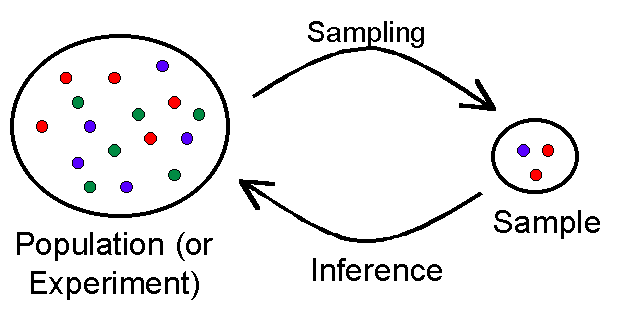
\includegraphics[height=0.4\textheight]{Inf_I/PopulationSample}
  \end{center}
\end{frame}

\begin{frame}{Relembrando}
  \begin{definition}
    Um \alert<1>{parâmetro} é uma variável numérica que representa uma
    característica da \alert<1>{população}.
  \end{definition}
  \begin{definition}
    Uma \alert<2>{estatística} é uma variável numérica que representa
    uma característica da \alert<2>{amostra}.
  \end{definition}
\end{frame}

\begin{frame}{Relembrando}
  \begin{block}{População}
    \begin{displaymath}
      \mu = \frac{\sum x_i}{N}
    \end{displaymath}
    \begin{displaymath}
      \sigma^2 = \sqrt{\frac{\sum (x_i - \mu)^2}{N} }
    \end{displaymath}
  \end{block}
  \begin{block}{Amostra}
    \begin{displaymath}
      \bar{x} = \frac{\sum x_i}{n}
    \end{displaymath}
    \begin{displaymath}
      s^2 = \sqrt{\frac{\sum (x_i - \bar{x})^2}{n-1} }
    \end{displaymath}
  \end{block}
\end{frame}

\section{Estimadores}

\begin{frame}{Estimadores}
  \begin{itemize}
  \item Um \alert{estimador pontual} é uma estatística que será usada
    para inferir o valor do parâmetro
  \item Geralmente usamos um \^\ para designar o estimador. Assim
    $\hat{\theta}$ é o estimador de $\theta$
  \item É uma função (qualquer) dos dados: $\hat{\theta} = f(X_1, X_2, \ldots, X_n)$
  % \item Ou seja: qualquer estatística é um estimador pontual.
  \end{itemize}
\end{frame}

% \begin{frame}{Estimadores}
% Uma distinção importante:
%   \begin{itemize}
%   \item Um estimador é uma função de alguma amostra (variáveis
%     aleatórias $X_1, X_2, \ldots, X_n$)
%   \item Uma estimativa é a realização (valor) dessa função, dada uma
%     amostra específica (dados, $x_1, x_2, \ldots, x_n$)
%   \end{itemize}
%   \begin{example}
%     \begin{itemize}
%     \item População: Pesos de pessoas em uma cidade
%     \item Amostra: Pesos de pessoas em uma vizinhança
%     \item Estimador: proporção de obesos em uma amostra qualquer da
%       população
%     \item Estimativa: proporção de obesos em uma vizinhança específica
%     \end{itemize}
%   \end{example}
% \end{frame}

% \begin{frame}{Estimadores}
%   \begin{example}
%     Outros exemplos de estimadores para esses dados:\\
%     \begin{itemize}
%     \item Peso médio
%     \item Desvio padrão
%     \end{itemize}
%   \end{example}
% \end{frame}

% \begin{frame}{Estimadores}
%   \begin{itemize}
%   \item Mas podem haver vários estimadores possíveis para um mesmo parâmetro.
%   \item Como eles podem ser comparados?
%   \item Dados essas alternativas, como escolher um bom estimador para
%     o parâmetro?
%   \end{itemize}
% \end{frame}

\begin{frame}{Estimadores}
Características de um bom estimador são:
\begin{itemize}
\item Não-tendencioso (não-enviesado, não-viciado)
\item Consistência
\item Eficiência
\end{itemize}
\end{frame}

\begin{frame}{Estimadores}
  \begin{definition}
    Um estimador é \alert{não viesado} (não tendencioso, não viciado)
    quando sua média (ou esperança) é o próprio valor do parâmetro.
  \end{definition}
  % \begin{example}
  %   \begin{displaymath}
  %     E[\hat{\mu}] = \mu
  %   \end{displaymath}
  % \end{example}
\end{frame}

% \begin{frame}{Estimadores}
%   \begin{definition}
%     Um estimador é \alert{consistente} quando sua variância diminui
%     conforme $n$ aumenta.
%   \end{definition}
%   % \begin{block}{Obs}
%   %   Diferença entre consistência e viés
%   % \end{block}
% \end{frame}

\begin{frame}{Estimadores}
  \begin{definition}
    Dados dois estimadores, o mais \alert{eficiente} é o que tem a
    menor variância.
  \end{definition}
\end{frame}

\begin{frame}{Estimadores}
  \begin{center}
    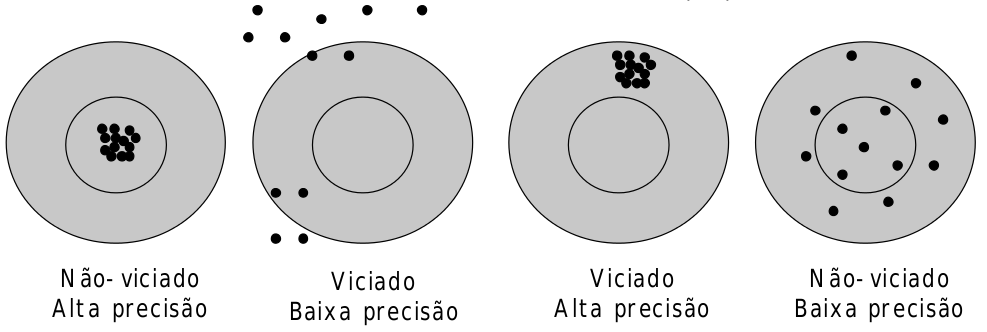
\includegraphics[width=\textwidth]{Inf_I/estimadores}
  \end{center}
\end{frame}

\section{Estimadores para a média}

\subsection{Estimadores pontuais para a média}

\begin{frame}{Estimadores pontuais para a média}
  \begin{block}{}
    O estimador $\hat{\mu}$ menos tendencioso para a média
    populacional $\mu$ é a média amostral $\bar{x}$.
  \end{block}
  \begin{displaymath}
    \hat{\mu} = \bar{x}
  \end{displaymath}
\end{frame}

\begin{frame}
  \begin{example}
    Uma estimativa pontual para a quantidade diária de cigarros por
    dia em uma população de fumantes pode ser obtida de uma amostra
    com 30 fumantes.
    \begin{displaymath}
      \hat{\mu} = \bar{x} = \frac{\sum x_i}{30} = 12.4
    \end{displaymath}
  \end{example}
\end{frame}

\subsection{Intervalos de confiança para a média}
\begin{frame}{Margem de erro para a estimativa da Média}
  \begin{itemize}
  \item Precisamos considerar o erro do estimador $\epsilon(\mu) =
    \mu - \hat{\mu}$
  \item Mas se tivéssemos $\mu$, não precisaríamos de $\hat{\mu}$!
  \item Assim, precisamos de um outro tipo de estimador, que leve em
    conta uma margem de erro em torno da estimativa pontual
  \end{itemize}
\end{frame}

\begin{frame}{Estimadores Intervalares para a Média}
  \begin{definition}
    Chamamos de \alert{nível de confiança} $c$ a probabilidade de que
    o parâmetro esteja dentro do intervalo
  \end{definition}
  \begin{definition}
    Um \alert{estimador intervalar} é um intervalo torno do estimador
    pontual, considerando uma \alert{margem de erro} $E$ e o nível de
    confiança $c$ da estimativa.
  \end{definition}
\end{frame}

\begin{frame}{Intervalos de Confiança para a Média}
  \begin{itemize}
  \item Níveis de confiança usuais: 90\%, 95\% e 99\%.
  \item Associados a esses níveis de confiança temos os respectivos
    valores críticos $z_c$ da distribuição normal padrão
  \item Valores tabelados: $z_c(0.90) = 1.645$, $z_c(0.95)=1.96$ e
    $z_c(0.99)=2.575$.
  \end{itemize}
\end{frame}

% \begin{frame}{Intervalos de Confiança para a Média}
%   \begin{definition}
%     Dado o nível de confiança $c$, 
%   \end{definition}
% \end{frame}

\begin{frame}{Intervalos de Confiança para a Média}
  Se a amostra é grande ($n \ge 30$) temos boas condições analíticas!
  Pelo Teorema Central do Limite (TCL):
  \begin{itemize}
  \item podemos aproximar uma distribuição normal (contínua) pela
    binomial (discreta)
  \item podemos aproximar o desvio-padrão populacional $\sigma$ por
    pelo desvio-padrão amostral $s$
  \item Calculamos assim a margem de erro $E$ como
    \begin{displaymath}
      E = \frac{z_c \cdot s}{\sqrt{n}}
    \end{displaymath}
  \item O Intervalo de Confiança fica então
    \begin{displaymath}
      \bar{x} \pm E = (\bar{x}-E , \bar{x} +E)      
    \end{displaymath}
  \end{itemize}
\end{frame}

\begin{frame}{Interpretação}
  \begin{block}{}
    Dizemos que o intervalo tem, por exemplo, 95\% de chance de
    conter o verdadeiro valor da média populacional.
  \end{block}
  \begin{itemize}
  % \item Isso é diferente de dizer que a média de 95\% de estar dentro
  %   do IC
  \item Obs: A média é um valor fixo, está contido ou não.
  \end{itemize}
\end{frame}

\begin{frame}{Exercício}
  \begin{block}{Exercício}
    Num estudo para descrever o perfil dos pacientes adultos atendidos
    no ambulatório de um posto de saúde, uma amostra de 70 pacientes
    adultos foi selecionada ao acaso entre o total de pacientes
    atendidos no posto durante os últimos três anos, coletando-se dos
    prontuários desses pacientes dados relativos à idade, à
    escolaridade e a outros fatores de interesse.\\

    Para a variável idade, observou-se uma média amostral de 36.86
    anos com um desvio padrão amostral de 17.79 anos.
  \end{block}
\end{frame}

\begin{frame}{Exercício}
  \begin{block}{Exercício}
    \begin{enumerate}
    \item Defina a população e a amostra.
    \item Forneça uma estimativa pontual, um intervalo de 90\% de
      confiança e um intervalo de 95\% de confiança para a idade média
      dos adultos atendidos neste ambulatório nos últimos três
      anos. Interprete e compare os intervalos de confiança.
    \end{enumerate}
  \end{block}

  \begin{block}{}
    \begin{columns}
      \begin{column}{5cm}
    \begin{displaymath}
      E = \frac{z_c s}{\sqrt{n}}
    \end{displaymath}
    \begin{displaymath}
      z_c (95\%) = 1.96
    \end{displaymath}
    \begin{displaymath}
      z_c (90\%) = 1.645
    \end{displaymath}
  \end{column}
  \begin{column}{5cm}
    \begin{displaymath}
      \bar{x} = 36.86
    \end{displaymath}
    \begin{displaymath}
      s = 17.79
    \end{displaymath}
    \begin{displaymath}
      n = 70
    \end{displaymath}
  \end{column}
\end{columns}
\end{block}
\end{frame}

\begin{frame}{Exercício}
  \begin{block}{Solução}
    \begin{itemize}
    \item IC de 90\% (c=0.90)
    \begin{displaymath}
      E = \frac{z_c s}{\sqrt{n}} = \frac{1.645 \times 17.79}{\sqrt{70}}
      \approx 3.50
    \end{displaymath}
    \begin{displaymath}
      IC_{0.90} = \bar{x} \pm E = 36.86 \pm 3.50 = (33.36 , 40.36)
    \end{displaymath}
  \item IC de 95\% (c=0.95)
    \begin{displaymath}
      E = \frac{z_c s}{\sqrt{n}} = \frac{1.96 \times 17.79}{\sqrt{70}}
      \approx 4.17
    \end{displaymath}
    \begin{displaymath}
      IC_{0.95} = \bar{x} \pm E = 36.86 \pm 4.17 = (32.69 , 41.03)
    \end{displaymath}
  \end{itemize}
\end{block}
\end{frame}

\begin{frame}{Exercício}
  \begin{block}{Comparando os ICs}
    \begin{displaymath}
      IC_{0.90} = (33.36 , 40.36)
    \end{displaymath}
    \begin{displaymath}
      IC_{0.95} = (32.69 , 41.03)
    \end{displaymath}
    Pergunta: Qual estimativa intervalar tem \alert{maior precisão}?\\

    Ou: Para qual nível de confiança o IC é \alert{menor}?
  \end{block}
  % \begin{block}{Amplitudes dos ICs}
  %   \begin{displaymath}
  %     40.36 - 33.36 = 7
  %   \end{displaymath}
  %   \begin{displaymath}
  %     41.03 - 32.69 = 8.34
  %   \end{displaymath}
  % \end{block}
\end{frame}

\section{Estimadores para proporções}

\subsection{Estimadores pontuais para proporções}

\begin{frame}{Estimadores pontuais para proporções}
  \begin{itemize}
  \item Para variáveis categóricas, é conveniente considerar
    a proporção da amostra que satisfaz o critério desejado
  \item Se $x$ é o número de sucessos na amostra, o estimador pontual
    da proporção populacional é:
    \begin{displaymath}
      \hat{p} = \frac{x}{n}
    \end{displaymath}
  \end{itemize}
\end{frame}

\begin{frame}{Estimadores pontuais para proporções}
  \begin{example}
    \begin{itemize}
    \item População: fumantes no prédio
    \item Parâmetro: $p=$ proporção de fumantes no prédio
    \item Estimativa: $\hat{p}=$ proporção de fumantes na sala
    \end{itemize}
  \end{example}
\end{frame}

\subsection{Intervalos de confiança para proporções}

\begin{frame}{Intervalos de confiança para proporções}
  \begin{itemize}
  \item Podemos construir um intervalo de confiança de maneira análoga
    à usada para médias
  \item A margem de erro considera a proporção de sucessos $\hat{p}$ e
    a proporção de fracassos $\hat{q} = 1- \hat{p}$
    \begin{displaymath}
      E = z_c \sqrt{\frac{\hat{p}\hat{q} }{n}}      
    \end{displaymath}
  \item Essa aproximação é válida sempre que $n\hat{p}\ge 5$ e
    $n\hat{q}\ge 5$ (amostras grandes)
  \item O IC fica então $\hat{p} \pm E = (\hat{p} -E, \hat{p} +E)$
  \end{itemize}
\end{frame}

\begin{frame}{Exercício}
  \begin{block}{Exercício}
    Num estudo para descrever o perfil dos pacientes adultos atendidos
    no ambulatório de um posto de saúde, uma amostra de 70 pacientes
    adultos foi selecionada ao acaso entre o total de pacientes
    atendidos no posto durante os últimos três anos, coletando-se dos
    prontuários desses pacientes dados relativos à idade, à
    escolaridade e a outros fatores de interesse.\\

    Para a variável escolaridade, observou-se que 19 pacientes da
    amostra eram analfabetos.
  \end{block}

\end{frame}

\begin{frame}{Exercício}
  \begin{block}{Exercício}
    \begin{enumerate}
    \item Forneça uma estimativa pontual, um intervalo de 90\% de
      confiança e um intervalo de 95\% de confiança para proporção de
      analfabetos dentre os adultos atendidos neste ambulatório nos
      últimos três anos. Interprete e compare os intervalos de
      confiança.
    \end{enumerate}
  \end{block}

  \begin{block}{Exercício}
    \begin{columns}
      \begin{column}{5cm}
        \begin{displaymath}
          E = z_c \sqrt{\frac{\hat{p}\hat{q} }{n}}
        \end{displaymath}
        \begin{displaymath}
          z_c (95\%) = 1.96
        \end{displaymath}
        \begin{displaymath}
          z_c (90\%) = 1.645
        \end{displaymath}
      \end{column}
      \begin{column}{5cm}
        \begin{displaymath}
          \hat{p} = \frac{19}{70} \approx 0.27
        \end{displaymath}
        \begin{displaymath}
          \hat{q} = 1-0.27 = 0.73
        \end{displaymath}
        \begin{displaymath}
          n = 70
        \end{displaymath}
      \end{column}
    \end{columns}
  \end{block}
\end{frame}

\begin{frame}{Exercício}
  \begin{block}{Solução}
    \begin{itemize}
    \item IC de 90\% (c=0.90)
      \begin{displaymath}
        E = z_c \sqrt{\frac{\hat{p}\hat{q} }{n}} = 1.645 \sqrt{\frac{0.27
            \times 0.73}{70} } \approx 0.09
      \end{displaymath}
      \begin{displaymath}
        IC_{0.90} = 0.27 \pm 0.09 = (0.18 , 0.36)
      \end{displaymath}
    \item IC de 95\% (c=0.95)
      \begin{displaymath}
        E = z_c \sqrt{\frac{\hat{p}\hat{q} }{n}} = 1.96 \sqrt{\frac{0.27
            \times 0.73}{70} } \approx 0.10
      \end{displaymath}
      \begin{displaymath}
        IC_{0.95} = 0.27 \pm 0.10 = (0.17 , 0.37)
      \end{displaymath}
    \end{itemize}
  \end{block}
\end{frame}

\section{Tamanhos de amostras}

\begin{frame}{Tamanho da amostra (médias)}
  \begin{itemize}
  \item Podemos aumentar a precisão do IC sem diminuir o nível de confiança
  \item Para isto, basta aumentar o tamanho da amostra
  \item Revirando a fórmula da margem de erro $E$, temos:
  \end{itemize}
\end{frame}

\begin{frame}{Tamanho da amostra (médias)}
  \begin{displaymath}
    E = \frac{z_c \cdot s}{\sqrt{n}} 
  \end{displaymath}
  \uncover<2->{\begin{displaymath}
    \sqrt{n} = \frac{z_c \cdot s}{E}
  \end{displaymath}}
  \uncover<3->{\begin{displaymath}
    n =  \left(\frac{z_c \cdot s}{E}\right)^2
  \end{displaymath}}
\end{frame}

\begin{frame}{Exercício}
  \begin{block}{Exercício}
    Encontre o tamanho mínimo da amostra que dará uma margem de erro
    $E=2$ ao nível de confiança $c=0.95$ com desvio-padrão amostral $s=6.1$
    \begin{displaymath}
      n \ge \left(\frac{z_c \cdot s}{E}\right)^2
    \end{displaymath}
  \end{block}
  \begin{block}{Solução}
    \begin{displaymath}
      n \ge \left(\frac{1.96 \times 6.1}{2}\right)^2 \approx 35.7
    \end{displaymath}
    Portanto, $n$ precisa ser no mínimo $36$.
  \end{block}
\end{frame}

\section{Resumo}

\begin{frame}{Recapitulando}
  \begin{itemize}
  \item Quanto maior o nível de confiança (exigência), maior a
    amplitude do IC (menos precisão)
  \item Quanto maior o desvio-padrão (variabilidade) da amostra, maior
    a amplitude do IC (menos precisão)
  \item Quanto maior o tamanho da amostra (dados), menor a amplitude
    do IC (mais precisão)
  \item Dado um nível de confiança e uma margem de erro, podemos
    estimar o tamanho mínimo da amostra que gera este IC.
  \end{itemize}
\end{frame}

\end{document}
